\section{Étude de l'existant}
   Cette partie concerne le plus sur l'architecture globale des serveurs clouds de \gls{mdi}, leurs évolutions 
   au cours du temps ce qui éclaircira le besoin de la création du nouveau composant 
   point d entrée.  

   \subsection{Évolution des clouds \gls{mdi}}
   Les boîtiers \gls{obd} ont la particularité de s’intégrer dans tout type de véhicule et permettent
   l’émission, la réception, le traitement et la représentation de données diverses comme
   l'état de la batterie du véhicule, les données standards, les données du propriétaire du
   véhicule ou des données des capteurs du boîtier même (localisation GPS,
   l’accéléromètre, le gyroscope, la consommation de la batterie ...)et un tas d'autres informations complémentaires.
   Ces données là ont besoin d'être traité pour pouvoir en sortir de l'information utile, d'où le besoin de services divers, regroupés 
   dans un cloud. \\ 
     \begin{figure}[ht]
        \centering
        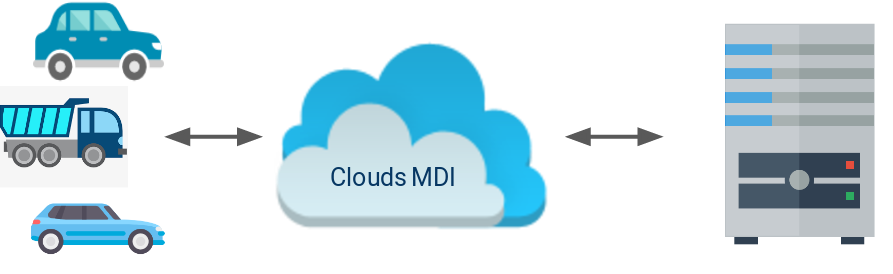
\includegraphics[scale=0.4]{\images/existant2.png}
        \caption{Communication avec le cloud}
    \end{figure}
        
        Le Cloud collecte les informations des véhicules récoltés par ces produits intégrés, traite et stocke ces 
   derniers et communique avec les serveurs clients externes.


    \subsubsection{Le premier Cloud de MDI}
       
    
         Le CloudConnect - ou \gls{CC} - est le premier cloud fait maison de \gls{mdi} qui englobe un ensemble 
        de services pour les clients. Créé en ..et hébergés dans des serveurs d'OVH, \gls{CC} traite 
        jusqu'à présent un nombre important du traitement des données. CloudConnect propose également un écosystème d’applications partenaires (gestion de flottes, ecodriving…) 
        mais aussi des services connectés par l’intermédiaire de partenaires. \\ [0.2cm]
        L'architecture globale de ce cloud est présenté par le schema de la figure \ref{fig:cc} de la page \pageref{fig:cc}.

        \begin{figure}[ht]
            \centering
            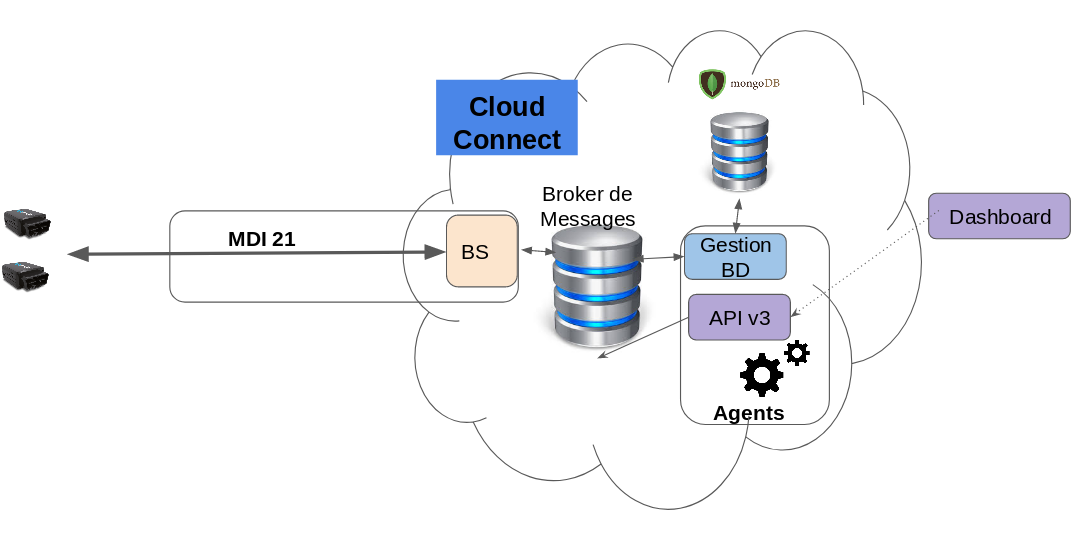
\includegraphics[scale=0.4]{\images/cc.png}
            \caption{L'architecture de CloudConnect - \gls{CC}}
            \label{fig:cc}
        \end{figure}

        Pour des raisons de confidentialité ce schema a été simplifié. Néanmoins, il présente les principaux composants de CloudConnect. 
        Parmi ces coposants on trouve : \\
        \begin{itemize}
            \renewcommand{\labelitemi}{$\bullet$}
            \item  un \textbf{\gls{BS}} qui est le composant d'échange de messages entre le cloud et 
            les OBD. Il présente le point d'entrée du cloud et représente le composant en question. Il supporte \gls{mdi21}, le protocole
            de l'entreprise conçu pour la communication entre boîtiers et Cloud.
            Nous détaillerons bien ce composant à la fin de ce chapitre.        \vspace{0.2cm}

            \item  un  \textbf{ broker de messge :} pour les systèmes Big Data. C'est un système distribué très répandu dans le domaine de BigData centralisant le flux de données provenant 
            des différents systèmes de l'entreprise tout en gardant le découplage entre les systèmes producteurs de ceux consommateurs de données.\\ 
            Le point fort de cet outil est sa capacité de supporter des débits très importants que ce soit pour 
            la publication ou la lecture des données. D'autres part, ce broker permet la consommation des données en temps réel et en mode batch, 
            en persistant les données. Il est à noter que les données ne sont pas stockés dans ce système, ils sont là jusqu'à leurs consomattion. 
            D'où le besoin d'une base de données.         \vspace{0.2cm}

            \item une \textbf{base de données NoSQL} orienté documents pour le stockage des données jusqu'à 3 mois.         \vspace{0.2cm}

            \item  un ensemble de services qui sont accéder à partir de \textbf{API-V3}:         \vspace{0.2cm}

            \item un \textbf{dashboard} pour l'affichage des données et l acces visuel 
            des services au clients 
        \end{itemize}
        \vspace{0.2cm}


        Il est bien de noter que l'équipe serveur de \gls{mdi} veille à ce que sa politique de récupération des données 
        respecte la nouvelle réglementation de \gls{gdpr}\cite{gdpr}. 
      
    
    \subsubsection{De \gls{CC} à \gls{CN}}

       Bien que le CloudConnect paraît complet. Il présente quelques problématiques au niveau de : 
       \begin{itemize}
        \renewcommand{\labelitemi}{$\bullet$}
            \item \textbf{Développement des agents :} Un Framework interne est utilisé pour simplifier le développement des différents 
        agents en langage ruby. Ce framework fournit un ensemble de fonctions qui permettent, entre autres, d’accéder au 
        courtier de messages en lecture et en écriture. Concernant les agents à état, le framework ne fournit pas 
        de mécanismes pour simplifier la gestion de leurs états. La gestion de l’état est donc laissée aux développeurs.\\[0.3cm]
            \item \textbf{Déploiement des agents :} les agents sont exécutés de manière parallèle. En d’autres termes, un agent peut avoir 
        plusieurs instances déployées dans différentes machines. Les différentes instances d’un même agent partagent 
        le traitement du flux des événements mais ne communiquent pas entre eux. Le déploiement ainsi que la maintenance 
        d’un agent se traduisent par une mise-à-jour des fichiers de configuration des machines exécutant l’agent via le logiciel Chef.\\ [0.3cm]
    \end{itemize}

         Comme solution à ces problèmes, \gls{mdi} a eu recours à la création d‘un autre Cloud afin de revoir l’architecture 
        logicielle et technique de CloudConnect afin de simplifier le développement des agents, leurs déploiements 
        ainsi que leurs maintenances et de permettre à des développeurs externes de l’entreprise de coder leurs propres agents.\\
        L'entreprise a créé alors sa propre infrastructure adaptée aux données de la télématique appelée « CloudNext » - ou  \gls{CN} 
        dont l’objectif est de se diriger vers une infrastructure orientée containers qui rend plus facile l’intégration de 
        solutions développées par les clients de l’entreprise et permet de diversifier ses activités.\\ [0.3cm] 
        L'architecture simplifié du \gls{CN} est présenté par la figure \ref{fig:cn} dans la page \pageref{fig:cn}.


        \begin{figure}[h!]
            \centering
            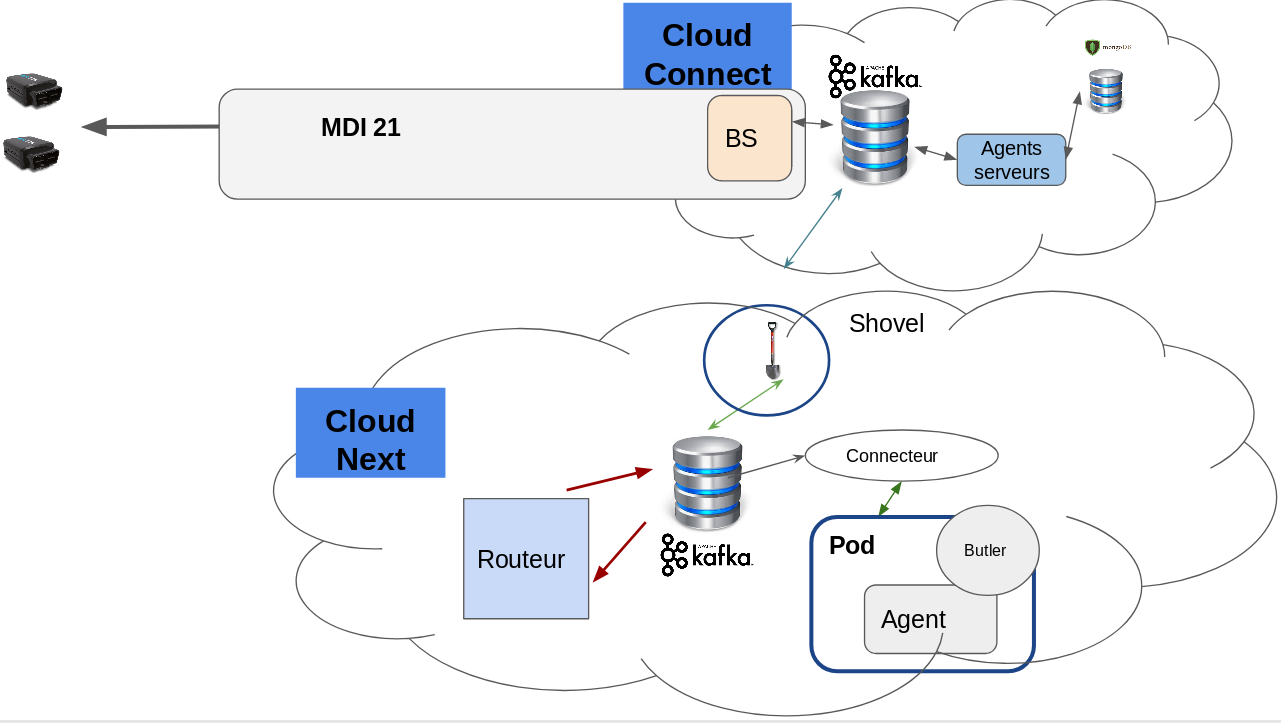
\includegraphics[scale=0.4]{\images/cn.png}
            \caption{L'architecture du cloud avec CloudNext}
            \label{fig:cn}
        \end{figure}

        \vspace{0.2cm}

        Dans le nouveau cloud on trouve d'autres composants nouveaux. 
        Parmi eux on trouve : \\[0.3cm]
        \begin{itemize}
            \renewcommand{\labelitemi}{$\bullet$}
                \item \textbf{Shovel :} Il traduit les informations du format “MessagePack” au format “Protobuf”.\\
                \item \textbf{Routeur :} Il assigne chaque track à un agent.\\
                \item \textbf{Connecteur :} Il gère les états des stateful agents\\ 
                \item \textbf{Pod :} Les pods de Kubernetes\\
                \item \textbf{Butler :} \\
                \item \textbf{Agent :} Un service Cloud \\
                \item docker custom registery
            \end{itemize} 

            Pour faciliter la communication entr les agents, \gls{CC} migre vers un format de message de MsgPack  vers ProtoBuffer 

            \vspace{0.2cm}

            ***********Expliquer différence entre MsgPack et Protocole  Buffer *******

    \subsection{le BS \gls{mdi21} de plus pres}

        Redis , Indigen ..., fonctionnalités \\
       

        le \gls{BS} est le service de communication. Il présente le point d'entrée des boîtiers au CloudConnect. 
            Multiple instances sont lancés sur des serveurs host différents pour assurer la balance de la charge 
            et éviter les \textit{Single Point Of Failure}. \\
        Cet agent est codé en Erlang, c’est un problème pour la garantie de la maintenance future du composant.
        Erlang perds de son intérêt pour 2 raisons:
            L'élasticité de la VM n’est plus utile avec Docker et Kubernetes
            Le chargement à chaud des nouvelles versions et la coexistence avec les anciennes version est aussi 
            disponible avec Docker et Kubernetes

        Le BS écrit dans RQueue et le Shovel copie de RQueue vers Kafka. donc il n'écrit pas directement dans le broker de message de CloudNext.


        Les informations de session sont dans redis (socket permanente).
        Les informations statiques (fields, channels, paramètres des accounts) sont récupérés depuis les apis (web services) - c’est une action rare.
        De plus les changements en DB sont notifiés au BS via Kafka.

        \subsubsection{Format de données}
        Les informations remontées par les boîtiers sont considérées comme des évènements. Ces événement peuvent contenir 
        des tracks , des messages et/ou des présences.\\
        \begin{itemize}
            \renewcommand{\labelitemi}{$\bullet$}
            \item \textbf{Track :} informations géolocalisées envoyés depuis le boîtier au Cloud et qui sont les données remontés des capteurs traités par les boîtiers. \\
            \item \textbf{Message :} informations plus complété qui se dirige vers un channel précis, invoqué depuis le serveur vers le boîtier.\\
            \item \textbf{Présence :} état du boîtier, si il est connecté au serveur ou pas.\\
        \end{itemize}

        \subsubsection{Transmission boitier-serveur }
        La transmission se fait en utilisant le protocole \gls{mdi21}. \gls{mdi21} est une logique in-house de séquence 
        ainsi qu’un encodage décrit en \gls{asn1}\\
        Ce protocole fonctionne en TCP et en UDP. L’UDP n’est que rarement utilisé étant 
        donné que les opérateurs téléphonique ne le favorise pas, voire rendent son utilisation impossible correctement.
        L’utilisation d’UDP nécessite en parallèle un lien TCP.\\
        Le lien est à l’initiative du boîtier,c'est à dire que le boîtier qui doit se connecter en premier au serveur en passant par le \gls{BS}
        La sécurité du lien est demandée par le boîtier au serveur et supporte les modèles récents (TLS 1.2).\\
        Une limitation actuelle, c’est que les transaction ne sont pas identifiées et que le serveur ne peut donc pas indiquer 
        au boîtier un index unique du dernier track traite. De ce fait, le boîtier re-envoi tous les track qui n’ont pas été 
        reconnu et on a des rejeu de données.